\documentclass[8pt]{beamer}

\usepackage[utf8]{inputenc}
\usepackage{default}

\usetheme{Madrid}

\author[J. Pela]{João Pela}
\title[BLA]{Bla}
\institute[ICL]{Imperial College London}
\date{2014-11-03}


\begin{document}

% ###################################################
\begin{frame}{Gen Met Vs Reco MET I}
 
\begin{columns}

\column[t]{0.45\linewidth} 
 
\begin{block}{\begin{tiny}MC Filter: Vectorial sum of neutrino $E_T$\end{tiny}}


\begin{itemize}
  \item $\sum E_\perp(\vec{\nu}) > 40$ $GeV$
\end{itemize}

\end{block}

\begin{block}{\begin{tiny}MC Filter: Dijet Filter\end{tiny}}

  \begin{itemize}
    \item Select jets with:
    \begin{itemize}
      \item $p_\perp>20$ $GeV$
      \item $|\eta|<5.0$
    \end{itemize}
    \item From selected jets at least one pair with:
    \begin{itemize}
      \item $m_{jj}>700$ $GeV$
      \item $\Delta\eta>3.2$
    \end{itemize}  
  \end{itemize}

\end{block}

\column[t]{0.45\linewidth} 

\begin{block}{QCD Inc 80-600 $GeV$}
 
\centering
 
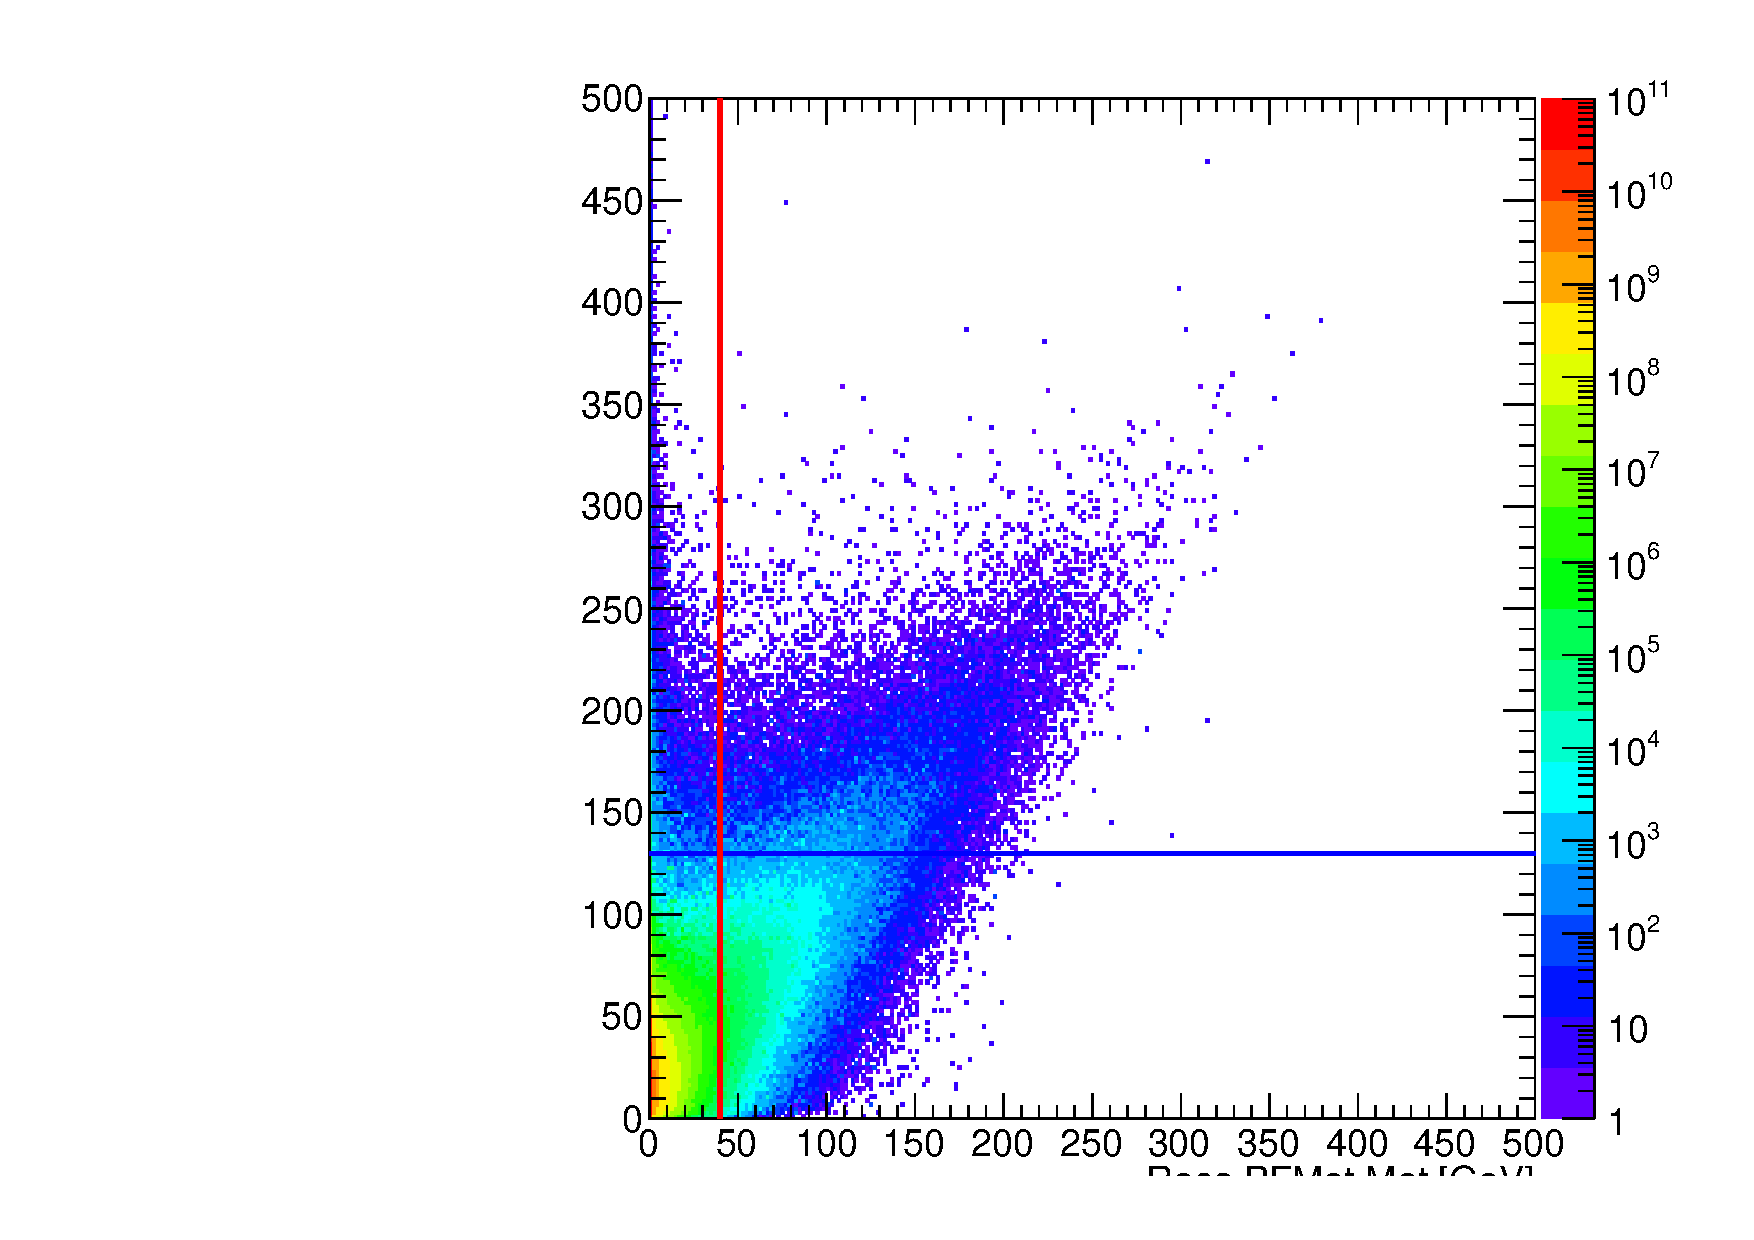
\includegraphics[width=0.7\linewidth]{img/MC_QCDIncAll_GenVsReco_met}
 
There 2 distict population events: real and fake met.
 
\end{block}

\end{columns}

\begin{block}

\centering
\resizebox{0.8\linewidth}{!}{
\begin{tabular}{|c|r|c|r|c|c|}
\hline
Sample          &       Ev. Gen. & Filter Eff. &  Events &  XS $[pb]$ & Eq. Lumi. $[fb^{-1}]$ \\
\hline \hline
QCD-Pt-80to120  & 39376000000 &    0.000049 & 1614416 &  1033680 &  38.09 \\
QCD-Pt-120to170 &  7000000000 &    0.000283 & 2051000 & 156293.3 &  44.79 \\
QCD-Pt-170to300 &  1375000000 &    0.000987 & 1391500 & 34138.15 &  40.28 \\
QCD-Pt-300to470 &    80000000 &    0.002659 &  207840 & 1759.549 &  45.47 \\
QCD-Pt-470to600 &    25000000 &    0.004127 &  104675 & 113.8791 & 219.53 \\
\hline
\end{tabular}
}

\end{block}

\end{frame}

\end{document}


